\chapter{Financial background}

Derivatives have become important in finance in the last 30 years with futures and options actively traded worldwide. The derivatives market is much bigger than the stock market when underlying assets are measured. Derivatives can be used for hedging, speculation or arbitrage as they transfer a wide range of risks in the economy from one entity to another. A \textit{derivative} is a financial instrument with a value that derives from the value of some other basic underlying asset.~\cite[pg.1]{ofod}

\section{Options}
We will focus on one type of derivatives - \textit{options}. These are contracts that give the holder the right to buy or sell the underlying asset. This is in contrast with other derivatives - \textit{forwards} and \textit{futures}, where the holder is obligated to buy or sell the underlying asset.

There are two types of options. A \textit{call option} gives the holder the right to buy the underlying asset by a certain date for a certain price. A \textit{put option} gives the holder the right to sell the underlying asset by a certain date for a certain price. The price in the contract is called \textit{strike price} and the expiration date is called \textit{maturity}. Options that can be exercised at any time before maturity are known as \textit{American options} and options that can be exercised only on the expiration date itself are known as \textit{European options}. One contract usually allows to buy or sell 100 shares.~\cite[pg.7-8]{ofod}

\paragraph{Example}
An investor spent 20.000 kr for an option to buy 100 Maersk shares for 9.600 kr each. The current price for Maersk stock is 9.440 kr as of March 15, 2018. If the price does not rise above 9.600 kr by the maturity, the investor does not exercise the option and loses 20.000 kr. However, if Maersk stock is priced at 10.000 kr when the option can be exercised, the investor is able to buy 100 shares for the strike price of 9.600 kr and immediately sell them for 10.000 kr. This will generate a profit of 40.000 kr minus the initial contract cost of 20.000 kr.

Table~\ref{table:option-sell} illustrates exercising this option at different dates. Even if the stock price rises above the strike price, the net profit might still be negative when the contract price is accounted for.  

\begin{table}[h]
\centering
\caption{Profit generated by a call option with strike price of 9.600 kr and contract price of $100 \times 200 = 20.000$ kr.}
\label{table:option-sell}
\begin{tabular}{|l|l|l|l|l|}
\hline
                       & March 2018    & June 2018 & Sept. 2018 & Dec. 2018 \\ \hline
Stock price (kr)       & 9.440         & 9.700     & 10.000         & 9.800         \\ \hline
Share sale profit (kr) & not exercised & 10.000    & 40.000         & 20.000        \\ \hline
Net profit (kr)        & -20.000       & -10.000   & 20.000         & 0             \\ \hline
\end{tabular}
\end{table}

\section{Bonds}
Bonds are a form of debt that allow companies or governments borrow money from investors. Most bonds periodically pay coupons (interest) to the holder. The principal payment (known as face value or par value) is paid at the end of bond's life.~\cite[pg.80]{ofod}

\paragraph{Zero rates}
Interest rate on an investment that starts today and lasts for $n$ years are called $n$-year zero-coupon interest rates. All the interest and principal is realized at the end. For example, an investment of 100\$ with a 5-year zero rate with continuous compounding at 5\% p.a. grows to~\cite[pg.80]{ofod}
\begin{equation*}
    100 \times e^{0.05 \times 5} = 128.40
\end{equation*}

\paragraph{Bond pricing}
The theoretical price of a bond can be calculated as the present value of all cash flows received by the holder. For example, there is a 2-year bond with 100\$ principal that pays coupons at the rate of 6\% semiannually. When the zero rates are as in table~\ref{table:zero-rates}, we can calculate the present value of the first coupon of 3\$ by discounting it at 5.0\% for 6 months, second coupon at 1 year and so on. Then the theoretical price of the bond is~\cite[pg.80-81]{ofod}
\begin{equation*}
    3e^{-0.05 \times 0.5} + 3e^{-0.058 \times 1.0} + 3e^{-0.064 \times 1.5} + 103e^{-0.068 \times 2.0} = 98.39
\end{equation*}

\begin{table}[h]
\centering
\caption{Zero rates used for bond pricing}
\label{table:zero-rates}
\begin{tabular}{|l|l|}
\hline
Maturity (years) & \begin{tabular}[c]{@{}l@{}}Zero rate (\%)\\ (continuously compounded)\end{tabular} \\ \hline
0.5              & 5.0                                                                                \\ \hline
1.0              & 5.8                                                                                \\ \hline
1.5              & 6.4                                                                                \\ \hline
2.0              & 6.8                                                                                \\ \hline
\end{tabular}
\end{table}

\paragraph{Bond yield}
A bond's yield is the single discount rate that gives a bond price equal to its market price. Continuing the pricing example, the yield $y$ can be computed as
\begin{equation*}
    3e^{-y \times 0.5} + 3e^{-y \times 1.0} + 3e^{-y \times 1.5} + 103e^{-y \times 2.0} = 98.39
\end{equation*}
This equation gets solved by setting $y = 6.76\%$.~\cite[pg.81]{ofod}

% ALGORITHM
\section{Algorithm and intuition}
\label{section:algorithm_and_intuition}
In order to achieve maximum parallelization efficiency, it is necessary to have a deep understanding of the algorithm itself. The book by John Hull\cite{ofod} provides a solid background on the topic, describing the mechanics of interest rates, markets, the need for binomial trees and how that has led to the use of trinomial trees. Chapter 30 further narrows the topic of using trinomial trees as a numerical method and introduces a step by step walk-through of applying the algorithm on a basic example. While some of the calculation details are omitted in the book, the authors provide references to previous articles\cite{npfits}\cite{uhwirt}, where they explain them. 

It is worth mentioning that the construction of a trinomial tree is a numerical method, but the example in the book is simplified by cutting the tree at a certain height and using analytic formulas to produce a concrete result for a specific financial instrument - a zero-coupon bond maturing at time $(m + 1) * \triangle t$ \cite[pg. 704]{ofod}. These formulas have found and proven to be effective by the authors of the book and the articles. While this simplification gives more precise results in the above mentioned specific case, constructing the entire tree and using all of the time steps can also give a good approximation for other financial instruments, even though being computationally harder. All the implementations of this thesis will be focused on the numerical approach.

The algorithm consists of two general steps. The first (forward propagation along the tree) is the construction of the trinomial tree in order to obtain a list of alpha values for each time step. These alphas are later used in the second step (backward propagation along the tree) to fit the bond prices and obtain the option value back at the root node of the tree. The input fed to the algorithm consists of a list of options, as for each option the information provided is its strike price, maturity, time step length, reversion rate\footnote{denoted as $a$ - determines the relative volatilities of long and short rates\cite[pg.9]{npfits}} and volatility\footnote{denoted as $\sigma$ - determines the overall level of volatility \cite[pg. 9]{npfits}}. The output is a list of option values for each inputted option. 

The following sub-chapters are focused primarily on the intuition behind the algorithm, with the sole purpose to provide the reader with a general overview of it. For this reason, many of the details and formulas of calculating specific values have been omitted, as they are thoroughly described in the book and the articles by Hull and White. As the model is best understood visually, we have included some of the supplementary images from the Hull and White book in order to support our algorithm explanation. 

\subsection{Forward propagation}
The forward propagation by itself consists of two stages. Furthermore, each of them computes different values on the same tree. While the tree height can grow indefinitely, depending on the number of time steps, Hull and White limit the width of the tree (TODO: FOR NO APPARENT REASON !!!), by setting $j_{min}$ and $j_{max}$\footnote{As the tree is 2 dimensional, in order to find and operate on every single node, it is necessary to use both its x and y coordinates, in this case denoted $i$ and $j$ respectively.} defining the maximum span of its width (where the root is located on $j=0$). Fig \ref{fig:treeconststage1} illustrates an example tree with indications of its width and height. 

\subsubsection*{Stage 1}
The first stage aims to construct a tree for a variable $R^*$ that is initially 0 and follows the process $dR^*=-aR^*dt + \sigma dz$ which is symmetrical about $R^*=0$\cite[pg.698-699]{ofod}. Together with $R^*$, $p_u$, $p_m$ and $p_d$ are calculated to match the respective up, mid and down probabilities that match the expected change and variance of the change in R over the next interval $\triangle t$. Since the width of the tree is limited between $j_{min}$ and $j_{max}$, some of the branching is calculated differently, thus $p_u$, $p_m$ and $p_d$ depend on the node position. Naturally the tree construction happens iteratively, node by node, starting from the root. In the end of the stage, this first tree will always have a symmetrical shape similar\footnote{Note that the width and height of the tree may differ based on the number of time steps and the maturity of the financial instrument} to fig.\ref{fig:treeconststage1}. 
\begin{figure}[H]
	\centering
	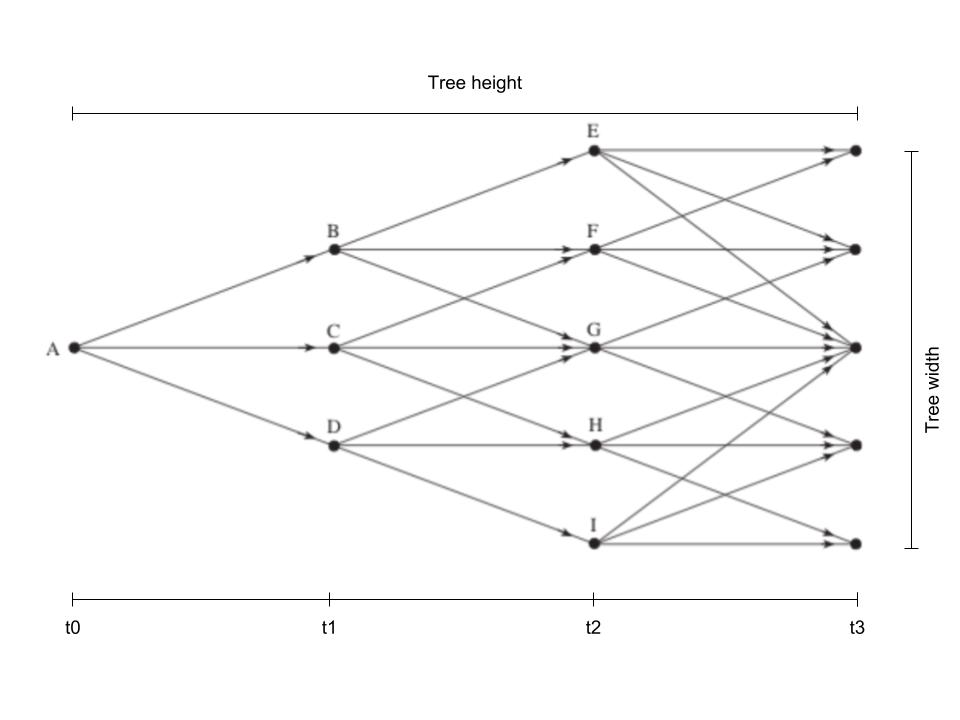
\includegraphics[width=0.8\textwidth]{img/treeconststage1wh.jpg}
	\caption{Example of the trinomial tree for $R^*$. Source: Modified by the authors, based on figure 30.8 \cite[pg. 699]{ofod}}
	\label{fig:treeconststage1}
\end{figure}

Some of the important properties of this tree include first of all its symmetry. The probabilities on the lower part of the tree will be the negative of the probabilities on the upper part of the tree, e.g. probability that node A reaches node D is minus the probability of node A reaching node B. Furthermore, also due to symmetry, all unique probabilities can be stored in an array of size the width of the tree, because e.g. the probability of node A reaching node B is the same as the probability of node C reaching node F and so on. Probabilities are used both in stage 2 of the forward propagation, but also in the backward propagation, thus it is necessary to preserve them to the end, if they are to be stored. Last but not least, the way probabilities are calculated is different on $j_{min}$ or $j_{max}$, because of the difference in branching. 

\subsubsection*{Stage 2}
In this stage, the rates at each node in the tree at each time step are shifted up by an amount - $\alpha$, chosen so that the revised tree correctly prices discount bonds \cite[pg. 6]{uhwirt}. This is done by defining $Q_{i,j}$ as the present value of a security that pays off \$1 if node (i, j) is reached and 0 otherwise. The starting point is to set $Q_{0,0}=0$ and $\alpha_0$ to the interest rate at time $\triangle t$.$Q$s at the next time step are then calculated by using the generalized formula \cite[pg.705]{ofod}:  
\begin{equation}
\begin{gathered}
\begin{aligned}
Q_{m+1, j} = \sum_k Q_{m,k}q(k,j)exp[-(\alpha_m+k\triangle r)\triangle t]
\nonumber
\end{aligned}
\end{gathered}
\end{equation}
Supposing that we are starting on step $m$, to calculate the $Q$s on step $m+1$, we need to have the alpha on step $m$. Furthermore, once the $Q$s on step $m+1$ have been calculated, they are used to also find the alpha on $m+1$ later. This leads to conclude that alphas and $Q$s are interrelated on each time step. Alphas are calculated using the generalized formula \cite[pg.703]{ofod}:
\begin{equation}
\begin{gathered}
\begin{aligned}
\alpha_{m} = \dfrac{\sum_{j=-n_m}^{n_m} Q_{m,j}e^{-j\triangle r\triangle t} - \ln{P_{m + 1}}}{\triangle t}
\nonumber
\end{aligned}
\end{gathered}
\end{equation}
At the end of this stage, the new tree will have a similar shape to the one shown in fig. \ref{fig:treeconststage2}. 
\begin{figure}[H]
	\centering
	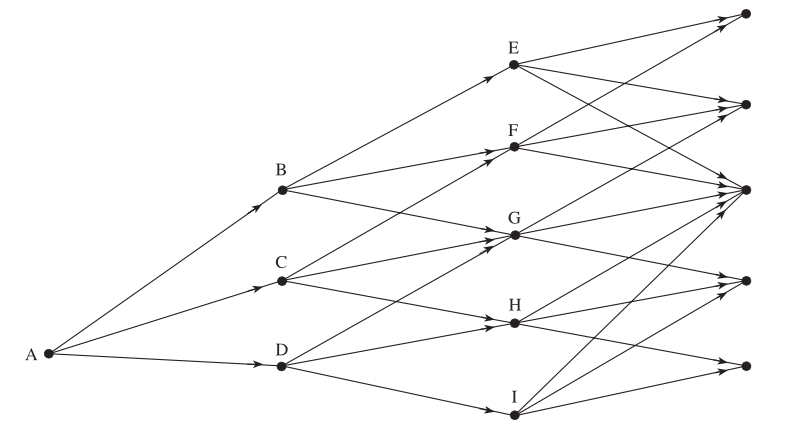
\includegraphics[width=0.8\textwidth]{img/treeconststage2.png}
	\caption{Example of the trinomial tree for $R$. Source: figure 30.9 \cite[pg. 702]{ofod}}
	\label{fig:treeconststage2}
\end{figure}
An important observation here is that the only outcome of this tree that is used in the backward propagation is the array of alphas. $Q$s are in this case intermediary values, used to compute the alpha on each step and for this reason, the $Q$ values do not need to be stored any longer once all alphas have been computed. 
\subsection{Backward propagation}
The backward propagation starts with an empty tree of the same width and height as the tree constructed during the forward propagation step. At each time-step the option payoff is computed as the discounted value of the expected value at the next step \cite[pg. 6]{uhwirt}. From this it follows that the nodes at time step $i$ (e.g. the nodes without assigned letters in figures \ref{fig:treeconststage1} and \ref{fig:treeconststage2} above) are the starting point of the backward propagation. Their values are set to \$100 and are used to compute the previous set of nodes (at time step $i-1$). That is done by discounting these values from the actual strike price of the option, by using the array of alphas and the array of probabilities, both computed during the forward propagation. It is important to note that determining the final option value also depends on the type of option (whether it is a put or a call option). These computations are iteratively done until reaching the root of the tree. This gives an approximation of the option value and is the output of the algorithm. 

An important observations to make is that both the forward and the backward propagation are composed of multiple aggregation operations, which is an overlay for multiple reads and writes of the data. There are two general ways to perform the reads and writes and it is important to optimize this process, specifically when trying to parallelize the algorithm in order to avoid data hazards. E.g. in order to compute the $Q$ value on node G in the forward propagation, values from nodes B, C and D have to be aggregated at node G. One approach to do that would be to calculate the values when being at each of the nodes B, C and D and write them to node G. This totals to a read and a write for each input node, or 3 reads and 3 writes. On the other hand, the value of Q can also be computed when at node G, by reading the values of B, C and D and adding them in one place before writing the result on node G. This takes 3 reads and 1 write operations. Since a write operations is more expensive, reducing the number of writes can have a crucial significance in parallel implementations, thus the second approach would always be preferable. In the backward propagation, the inverse intuition applies. E.g. the computation of the $call$ value at node C should be done while at node C, instead of while being at each of nodes F, G and H. While this should not produce any significant slowdown in the sequential implementation, or the one option per thread version, this thesis will focus on optimizing the writes in all of the implementations.

% Sequential IMPLEMENTATION
\section{Sequential implementation}
In order to better understand the algorithm, we have started with a basic sequential implementation of it in C++. While this step could be done in any language, we have chosen to work with C++, as it would allow us to re-use pieces of the code for the parallel CUDA implementations, described further in this paper. Running this version with a large number of options will likely result in a significant amount of computation time, however, the purpose of this implementation is rather a proof of concept that the algorithm produces correct approximations, as well as to provide a set of results, which can be used to test against with the other implementations. The sequential implementation code can be found under (TODO: INSERT CODE LOCATION HERE).

The algorithm described in the book is used to price one option at a time and the natural way to start a sequential implementation would be to create a single function that prices one option. Looping through all options in the data set and calling this function for each of them will then produce the end results. The pseudo-code below describes the approach we took for implementing a sequential version of the algorithm, based on the book and articles by Hull and White. Note that real is a data type that can either take the form of a double or a float, based on the necessary precision.

\begin{lstlisting}
for each option c:
    c:optionConstant -- the calculation of option constants
    -- option constants include:
    -- c.T:real -- option maturity
    -- c.t:int -- option length
    -- c.n:int -- option term step count
    -- c.dt:real -- 
    -- c.X:real -- option strike price
    -- c.dr:real --
    -- c.M:real -- 
    -- c.jmax: int -- max. j of the tree
    -- c.width: int -- the tree width
    
    Qs : real[c.width]
    QsCopy : real[c.width] 
    alphas[] : real[c.n + 1]
    
    jmin : -c.jmax
    
    Qs[c.jmax] = 1
    -- getYieldAtYear(t) returns the initial dt-period 
    -- interest rate
    alphas[0] = getYieldAtYear(c.dt) 
    
    -- iterates through nodes along tree height 
    -- (can be done as a gather if changed to 
    -- for i := 1 to to c.n included) 
    for i := 0 to c.n
        -- the highest allowed j index on step i
        jhigh:int = min(i, c.jmax)
        alpha:double = alphas[i]
        
        -- iterates through nodes along tree width
        -- between allowed j indexes on step i
        for j := -jhigh to jhigh
            Compute QsCopy on j+1, j and j-1 (scatter)
        end for
        
        -- iterates through the nodes along tree width
        -- between allowed j indexes on step i + 1
        jhigh1:int = min(i+1, c.jmax) 
        alpha_p1:real = 0
        for j := -jhigh1 to jhigh1
            Aggregate alpha_p1 based on QsCopy[j] 
        end for
        Compute alphas[i+1] based on alpha_p1
        
        Qs = QsCopy
        fill QsCopy with 0
    end for 
    
    Call:real[c.width]
    CallCopy:real[c.width]  
    
    for i := c.n-1 to 0 included
        jhigh = min(i, c.jmax)
        alpha:real=alphas[i]
        
        for j := -jhigh to jhigh
            jind:int=j-jmin
            Compute res based on j+1,j,j-1(gather)
            if i-th step is the maturity
                Call = max(c.X - res, 0)
            else
                Call = res
            endif    
        end for
        
        Call = CallCopy
        fill CallCopy with 0
    end for

    return Call[jmax] -- price approximation
    
end for each option c
\end{lstlisting}
The implementation iterates through all the options, constructs a trinomial tree for each of them and propagates back through it, obtaining the price approximations for each option and returning them in the end. The algorithm follows the intuition provided in the previous section - \ref{section:algorithm_and_intuition}.
    
As it can be seen from the pseudo-code, both the forward propagation and the backward propagation can be done differently, by applying combinations of scatter and gather. Despite that, a gather should always be preferable when dealing with parallelization, due to the reduced number of writes. It can prevent data races between threads and help improve the performance. The intuition behind this can be explained visually, as shown on fig. \ref{fig:scattervsgather}. A scatter can be characterized with reading values out of nodes reading their values and separately writing them to the same location, aggregating to its value. In the scatter example shown (left), a write operation (denoted with blue arrows) is performed from the three nodes (denoted with blue circles) to the same node, thus a total of 3 writes and 3 reads. A gather on the other hand happens when the values are read and aggregated together in one place. That is, on the right figure, the iterator is placed on mid right node, where three read operations are done (denoted with blue arrows), aggregated and followed by one write to the current node (denoted as with blue circle).

(TODO: MABYE WE SHOULD ALSO REPLACE THE SCATTER WITH GATHER ON THE SEQUENTIAL IMPL. AND SEE IF THAT GIVES ANY SPEEDUP BECAUSE OF THE WRITES? EVEN THOUGH WE DON'T CARE MUCH ABOUT THE SEQUENTIAL, OR MOVE THIS SECTION TO MULTIPLE OPTIONS PER THREAD BLOCK)

\begin{figure}[H]
	\centering
	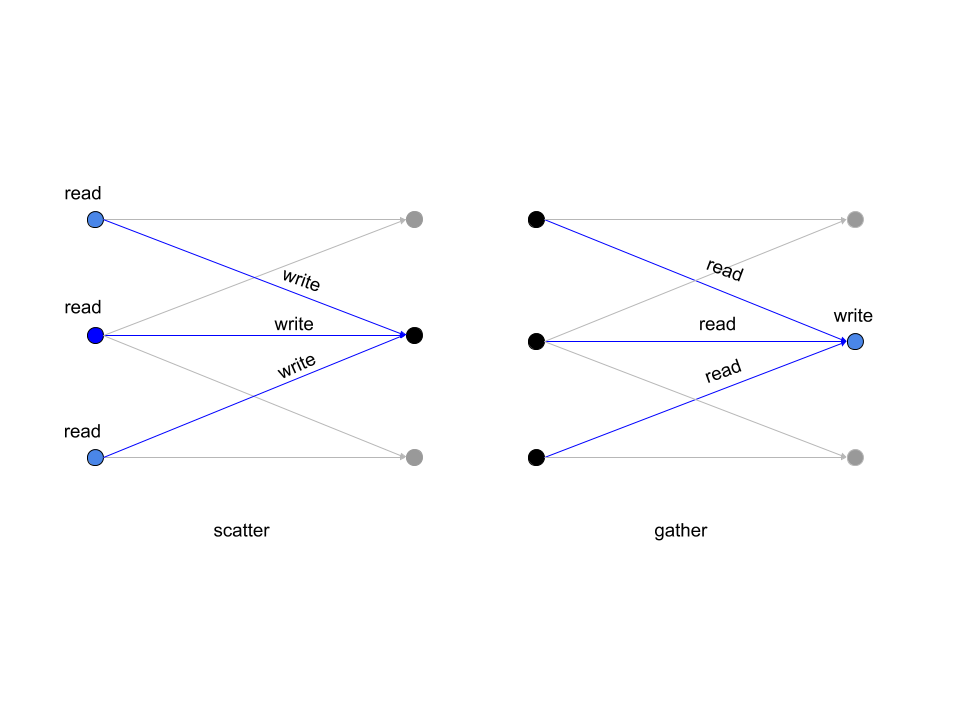
\includegraphics[width=0.8\textwidth]{img/scattervsgather.png}
	\caption{scatter vs. gather operations Source: Compiled by the authors}
	\label{fig:scattervsgather}
\end{figure}

(TODO: WRITE ABOUT CALCULATING ALPHAS IN THE FIRST LOOP)

It is important to notice that in a sequential implementation there are no data races, as everything is ran in one thread. Furthermore, it is not required to pre-allocate memory, while that would be necessary in a CUDA implementation. 

(TODO: WRITE ABOUT THE RESULTS WE OBTAINED FROM THIS IMPLEMENTATION)

\section*{Summary}
This chapter has provided the reader with an introduction to the financial background needed in order to proceed with accelerating the algorithm. It also provided a general overview of what the input of the algorithm is and the different steps it takes in order to compute the output. We have intentionally omitted most of the mathematics used in the algorithm, as well as explanations for what variables represent in financial terms, as that would be a repetition to what is also written in the book and the articles by Hull and White. The next chapter will introduce the first parallelization technique with CUDA - using one option per thread. It will aim at finding if and when that introduces any speedup over the sequential implementation, as well as how much that speedup will be.    